\section*{(14\textordfeminine\ aula) --- Problemas em 1D: Partícula Livre, Autovalores de $\hat{H}$ e Propagador}

\subsection*{Problemas em 1D (cap. 5)}

Nesse capítulo veremos como usar a MQ para descrever uma partícula que se move em 1D.

\subsubsection*{5.1 -- Partícula livre}

\begin{center}
\begin{tikzpicture}[scale=1]
    \draw[->, thick] (1.5,0.5) -- (2.5,0.5) node[midway, above] {$v$};
    \filldraw (1.5,0) circle (2.5pt) node[below] {$m$};
    \draw[->] (0,0) -- (6,0) node[right] {$x$};
\end{tikzpicture}
\end{center}

Aqui temos uma partícula que se move em 1D na \textbf{AUSÊNCIA DE QUALQUER TIPO DE FORÇA} (= partícula livre).

\begin{equation}
    \mathcal{L} = \frac{1}{2}m\dot{x}^2 \quad \Longrightarrow \quad H(x,p) = \frac{p^2}{2m}
\label{eq:aula14_lagrangiana_livre}
\end{equation}

A "solução" desse problema na Mecânica Clássica é:

\begin{equation}
    \begin{cases}
        \dot{x} = \dfrac{\partial H}{\partial p} = \dfrac{p}{m} \quad \Longrightarrow \quad x(t) = \dfrac{p\, t}{m} + x(0) \\[3mm]
        \dot{p} = -\dfrac{\partial H}{\partial x} = 0 \quad \Longrightarrow \quad p = \text{const} = p(0)
    \end{cases}
\label{eq:aula14_solucao_classica}
\end{equation}

Isso está OK se a partícula tiver uma massa apreciável, caso contrário você deve descrever a situação usando a MQ.

\begin{equation}
    \hat{H} = \frac{\hat{P}^2}{2m} \quad \text{é o operador Hamiltoniano}
\label{eq:aula14_hamiltoniano_op}
\end{equation}

O ket $\ket{\Psi(t)}$ mora no EV (espaço vetorial) das funções complexas de $x$.

\subsection*{Autovetores/Autovalores de $\hat{H}$ (calculados de 2 maneiras)}

\begin{equation}
    \hat{H}\ket{E} = E\ket{E}
\label{eq:aula14_autovalor_H}
\end{equation}

\subsubsection*{i) Projetando em $\bra{x}$}

\begin{equation}
    \bra{x}\frac{\hat{P}^2}{2m}\ket{E} = E\braket{x}{E}
\label{eq:aula14_projetando_x}
\end{equation}

\begin{equation}
    -\frac{\hbar^2}{2m}\frac{d^2}{dx^2}\psi_E(x) = E\,\psi_E(x)
\label{eq:aula14_eq_diferencial_E}
\end{equation}

\textbf{Atenção!} Isso é uma equação para determinar $E$ e $\psi_E(x)$. Os autovalores $E$ são obtidos da exigência de que $\psi_E(x)$ seja uma função do EV, isto é, $\psi_E(x)$ \textbf{NÃO PODE DIVERGIR EM $x = \pm\infty$}!

Funções do EV:
\begin{itemize}
    \item[(i)] normalizáveis, $\displaystyle\int_{-\infty}^{\infty} |\psi(x)|^2\, dx < \infty$
    \item[(ii)] não-normalizáveis, porém não divergentes em $\pm\infty$
\end{itemize}

\textbf{Caso $E < 0$:} teremos
\begin{equation}
    \psi_E'' = \left(\frac{2m|E|}{\hbar^2}\right)\psi_E \qquad \text{(EQ. de 2\textsuperscript{a} ordem!)}
\label{eq:aula14_eq_E_negativo}
\end{equation}
com solução
\begin{equation}
    \psi_E(x) = \alpha\, e^{+\sqrt{2m|E|/\hbar^2}\,x} + \beta\, e^{-\sqrt{2m|E|/\hbar^2}\,x}
\label{eq:aula14_solucao_E_negativo}
\end{equation}

Claramente isso não pertence ao EV.

\begin{equation}
    \boxed{E \text{ não pode ser negativo!}}
\label{eq:aula14_E_nao_negativo}
\end{equation}

\textbf{Caso $E > 0$:} teremos
\begin{equation}
    \psi_E'' = -\frac{2mE}{\hbar^2}\psi_E
\label{eq:aula14_eq_E_positivo}
\end{equation}

\fbox{\parbox{0.92\textwidth}{
\textbf{Obs:} como $\hat{H}$ é hermitiano sabemos que seus autovalores são reais; no entanto você pode provar isso observando que, para $E$ complexo, o produto $\psi_E(x)$ diverge no infinito.
}}

com solução
\begin{equation}
    \psi_E(x) = \alpha\, e^{i\sqrt{2mE/\hbar^2}\,x} + \beta\, e^{-i\sqrt{2mE/\hbar^2}\,x}
\label{eq:aula14_solucao_E_positivo}
\end{equation}
que é do tipo (ii) e pertence ao EV!

Essa análise é um exemplo de como os autovalores são descobertos. Concluímos que $E$ pode ser qualquer valor real e positivo (ou zero) (\textbf{ESPECTRO CONTÍNUO!}).

\begin{equation}
    \boxed{E \geq 0} \qquad \text{autovalores de } \hat{H}
\label{eq:aula14_espectro_H}
\end{equation}

Cada valor de $E$ é \textbf{DUPLAMENTE DEGENERADO}:
\begin{align}
    \braket{x}{E,+} &= \frac{1}{\sqrt{2\pi\hbar}}\, e^{i\sqrt{2mE/\hbar^2}\,x} \label{eq:aula14_ket_E_mais} \\
    \braket{x}{E,-} &= \frac{1}{\sqrt{2\pi\hbar}}\, e^{-i\sqrt{2mE/\hbar^2}\,x} \label{eq:aula14_ket_E_menos}
\end{align}
(não normalizados). Esses estados formam uma base do subespaço de energia $E$.

\fbox{\parbox{0.92\textwidth}{
\textbf{Obs:} essa escolha da constante de normalização não faz com que $\braket{E\alpha}{E'\beta} = \delta(E-E')\,\delta_{\alpha\beta}$.
}}

\subsubsection*{ii) Usando a base $\ket{p}$}

Aqui nem precisamos projetar $\hat{H}\ket{E} = E\ket{E}$ em $\ket{x}$. Como $\hat{H} = \dfrac{\hat{P}^2}{2m}$, segue que $\ket{p}$ é um autovetor de $\hat{H}$ com autoenergia $E$:

\begin{equation}
    \hat{H}\ket{p} = \frac{\hat{P}^2}{2m}\ket{p} = \frac{p^2}{2m}\ket{p}
\label{eq:aula14_H_ket_p}
\end{equation}

Veja que aqui descobrimos que $E \geq 0$ sem muito esforço. Qual a relação dos $\ket{p}$ com $\ket{E,+}$ e $\ket{E,-}$?

\begin{align}
    \ket{p = \sqrt{2mE}} &= \ket{E,+} \label{eq:aula14_p_E_mais} \\
    \ket{p = -\sqrt{2mE}} &= \ket{E,-} \label{eq:aula14_p_E_menos}
\end{align}

\fbox{\parbox{0.92\textwidth}{
Para obter essa identificação é que escolhemos as constantes de normalização acima como $(2\pi\hbar)^{-1/2}$.
}}

De fato, ambos os estados têm autovalor $E = p^2/2m$, e são a base, obtida acima, do subespaço de energia $E$.

\subsection*{Operador de evolução}

Conhecendo os autovalores/autovetores de $\hat{H}$ podemos montar o operador de evolução. Vimos que
\begin{equation}
    \hat{U}(t) = e^{-i\hat{H}t/\hbar}
\label{eq:aula14_U_def}
\end{equation}

Agora podemos usar $\hat{\mathbb{1}} = \displaystyle\int_{-\infty}^{\infty} dp\, \ket{p}\bra{p}$ (pois $\braket{p}{p'} = \delta(p-p')$) e obter

\begin{equation}
    \boxed{\hat{U}(t) = \int_{-\infty}^{\infty} dp\, \ket{p}\bra{p}\, e^{-ip^2t/2m\hbar}}
\label{eq:aula14_U_p}
\end{equation}
onde usei que $\hat{H}\ket{p} = \dfrac{p^2}{2m}\ket{p}$.

No entanto, \textbf{NÃO PODEMOS USAR} $\hat{\mathbb{1}} = \displaystyle\int_0^{\infty} dE \sum_{\alpha = +,-} \ket{E\alpha}\bra{E\alpha}$, uma vez que $\braket{E\alpha}{E'\beta} \neq \delta(E-E')\,\delta_{\alpha\beta}$, para exprimir $\hat{U}(t)$ como uma integral em $E$.

\subsubsection*{A identidade usando os $\ket{E\alpha}$}

\textbf{Atenção:} como não temos $\braket{E\alpha}{E'\beta} = \delta(E-E')\,\delta_{\alpha\beta}$ (onde $\alpha,\beta = +,-$) no nosso caso (pois a constante de normalização não foi escolhida para isso acontecer), \textbf{NÃO TEMOS}

\begin{equation}
    \hat{\mathbb{1}} \neq \int_0^{\infty} dE\, \underbrace{\left[\ket{E,+}\bra{E,+} + \ket{E,-}\bra{E,-}\right]}_{\text{``borboletas'' do subespaço de energia } E}
\label{eq:aula14_identidade_errada}
\end{equation}
como seria de esperar. Ao invés:

\begin{equation}
    \hat{\mathbb{1}} = \int_{-\infty}^{\infty} dp\, \ket{p}\bra{p} = \int_{-\infty}^{0} dp\, \ket{p}\bra{p} + \int_0^{\infty} dp\, \ket{p}\bra{p}
\label{eq:aula14_identidade_p_split}
\end{equation}

Mudando a variável para $p = -\sqrt{2mE}$ na 1\textsuperscript{a} integral e $p = +\sqrt{2mE}$ na 2\textsuperscript{a}:

\begin{equation}
    \hat{\mathbb{1}} = \int_0^{\infty} \sqrt{\frac{m}{2E}}\,\ket{E,-}\bra{E,-}\, dE + \int_0^{\infty} \sqrt{\frac{m}{2E}}\,\ket{E,+}\bra{E,+}\, dE
\label{eq:aula14_identidade_mudanca_var}
\end{equation}

\begin{equation}
    \hat{\mathbb{1}} = \int_0^{\infty} dE\, \sqrt{\frac{m}{2E}}\, \underbrace{\left[\ket{E,-}\bra{E,-} + \ket{E,+}\bra{E,+}\right]}_{\displaystyle\sum_{\alpha = +,-}}
\label{eq:aula14_identidade_E_final}
\end{equation}

\fbox{\parbox{0.92\textwidth}{
O fator $\sqrt{m/2E}$ não estaria aqui se $\braket{E\alpha}{E'\beta} = \delta(E-E')\,\delta_{\alpha\beta}$.
}}

\subsection*{Propagador}

Como vimos, um estado inicial qualquer $\ket{\Psi(0)}$, com função de onda conhecida $\braket{x}{\Psi(0)} = \Psi(x,0)$, evolui no tempo para

\begin{equation}
    \ket{\Psi(t)} = \hat{U}(t)\ket{\Psi(0)}
\label{eq:aula14_evolucao_ket}
\end{equation}

\begin{equation}
    \Longrightarrow \quad \braket{x}{\Psi(t)} = \int_{-\infty}^{\infty} dx'\, \bra{x}\hat{U}(t)\ket{x'}\braket{x'}{\Psi(0)}
\label{eq:aula14_evolucao_proj_x}
\end{equation}

\begin{equation}
    \Psi(x,t) = \int_{-\infty}^{\infty} dx'\, \underbrace{\bra{x}\hat{U}(t)\ket{x'}}_{U(x,x';t)\ \text{propagador}}\, \Psi(x',0) \tag{$*$}
\label{eq:aula14_propagador_def}
\end{equation}

\begin{equation}
    \bra{x}\hat{U}(t)\ket{x'} = \int_{-\infty}^{\infty} dp\, \braket{x}{p}\braket{p}{x'}\, e^{-i\frac{p^2}{2m}\frac{t}{\hbar}}
\label{eq:aula14_U_xx_passo1}
\end{equation}

\begin{equation}
    = \frac{1}{2\pi\hbar}\int_{-\infty}^{\infty} dp\, e^{i\frac{p(x-x')}{\hbar}}\, e^{-i\frac{p^2}{2m}\frac{t}{\hbar}}
\label{eq:aula14_U_xx_passo2}
\end{equation}

Aqui usamos
\begin{equation}
    \int_{-\infty}^{\infty} e^{-\alpha x^2 + \beta x}\, dx = \sqrt{\frac{\pi}{\alpha}}\, e^{\beta^2/4\alpha}
\label{eq:aula14_integral_gaussiana}
\end{equation}
válido mesmo que $\alpha$ e $\beta$ sejam complexos, \textbf{DESDE QUE} $\text{Re}\,\alpha \geq 0$.

Com isso

\begin{equation}
    \bra{x}\hat{U}(t)\ket{x'} = \frac{1}{2\pi\hbar}\left(\frac{\pi\, 2m\hbar}{i t}\right)^{1/2} e^{-\frac{(x-x')^2 m\hbar}{\hbar^2\, 2it}}
\label{eq:aula14_U_xx_passo3}
\end{equation}

\begin{equation}
    = \sqrt{\frac{m}{it\, 2\pi\hbar}}\; e^{i\frac{(x-x')^2 m}{2\hbar t}}
\label{eq:aula14_propagador_final}
\end{equation}

Para qualquer função de onda inicial $\Psi(x,0)$, o estado da partícula em $t$ será obtido da integração ($*$).

No caso particular do estado inicial ser
\begin{equation}
    \Psi(x,0) = \delta(x-a)
\label{eq:aula14_psi0_delta}
\end{equation}
(isso é incomum, dizer que a partícula está em um estado impróprio...), a integração é trivial e

\begin{equation}
    \Psi(x,t) = \int_{-\infty}^{\infty} dx'\, U(x,x';t)\, \delta(x'-a)
\label{eq:aula14_psi_xt_delta}
\end{equation}

\begin{equation}
    = U(x,a;t)
\label{eq:aula14_psi_xt_delta_resultado}
\end{equation}

Portanto você pode interpretar o propagador como a função de onda da partícula, no instante $t$, que, em $t=0$, estava infinitamente localizada em $x = x'$.

\subsection*{Evolução de um pacote gaussiano}

\begin{equation}
    \Psi(x,0) = \left(\frac{1}{\pi\Delta^2}\right)^{1/4} e^{i p_0 x/\hbar}\, e^{-x^2/2\Delta^2} \qquad \text{(função própria)}
\label{eq:aula14_pacote_gaussiano_inicial}
\end{equation}

Você pode verificar que o estado está normalizado
\begin{equation}
    \int_{-\infty}^{\infty} |\Psi(x,0)|^2\, dx = 1
\label{eq:aula14_normalizacao_pacote}
\end{equation}

\begin{center}
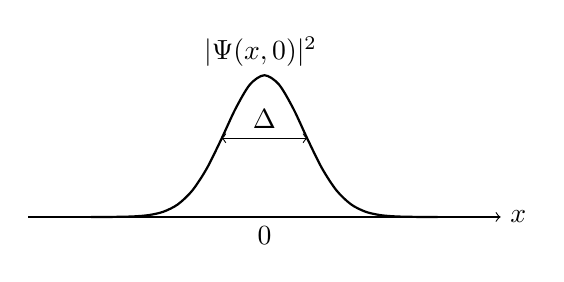
\begin{tikzpicture}[scale=1]
    \draw[->] (-3,0) -- (3,0) node[right] {$x$};
    \draw[domain=-2.2:2.2, smooth, variable=\x, thick] plot ({\x}, {1.8*exp(-2*\x*\x)});
    \draw[<->] (-0.55,1.0) -- (0.55,1.0) node[midway, above] {$\Delta$};
    \node at (-0.05,2.1) {$|\Psi(x,0)|^2$};
    \node[below] at (0,0) {$0$};
\end{tikzpicture}
\end{center}

\begin{equation}
    \aver{x} = 0 \qquad \Delta x = \frac{\Delta}{\sqrt{2}}
\label{eq:aula14_valores_esperados_x0}
\end{equation}

Você pode calcular facilmente $\aver{p} = p_0$ e $\Delta p = \dfrac{\hbar}{\sqrt{2}\Delta}$. Esse estado representaria uma partícula em uma região $\Delta$ em torno da origem e com velocidade em torno de $p_0/m$.

\begin{center}
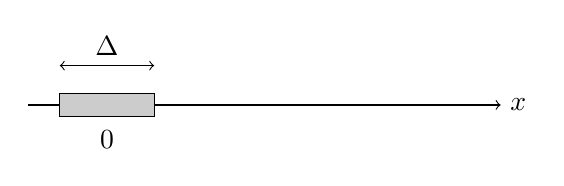
\begin{tikzpicture}[scale=1]
    \draw[->] (-1,0) -- (5,0) node[right] {$x$};
    \filldraw[fill=gray!40] (-0.6,-0.15) rectangle (0.6,0.15);
    \draw[<->] (-0.6,0.5) -- (0.6,0.5) node[midway, above] {$\Delta$};
    \node[below] at (0,-0.2) {$0$};
\end{tikzpicture}
\end{center}

\begin{equation}
    \frac{p_0}{m} - \frac{\Delta p}{m} < v < \frac{p_0}{m} + \frac{\Delta p}{m}
\label{eq:aula14_intervalo_velocidade}
\end{equation}

Em um instante $t$ posterior, o estado da partícula é descrito pela função de onda

\begin{equation}
    \Psi(x,t) = \int_{-\infty}^{\infty} \underbrace{\left(\frac{m}{it\, 2\pi\hbar}\right)^{1/2} e^{i\frac{(x-x')^2 m}{2\hbar t}}}_{U(x,x';t)}\; \underbrace{\left(\frac{1}{\pi\Delta^2}\right)^{1/4} e^{ip_0 x'/\hbar}\, e^{-x'^2/2\Delta^2}}_{\Psi(x',0)}\; dx'
\label{eq:aula14_psi_xt_integral}
\end{equation}

Veja que a integral é da forma $\displaystyle\int_{-\infty}^{\infty} e^{-\alpha x'^2 + \beta x'}\, dx'$ com

\begin{equation}
    \alpha = \frac{1}{2\Delta^2} - \frac{im}{2\hbar t} \qquad \text{e} \qquad \beta = -\frac{im}{\hbar t}x + \frac{ip_0}{\hbar}
\label{eq:aula14_alpha_beta}
\end{equation}

usando $\sqrt{\pi/\alpha}\, e^{\beta^2/4\alpha}$ para o resultado da integral (veja que $\text{Re}\,\alpha \geq 0$!):

\begin{equation}
    \Psi(x,t) = \left[\pi^{1/2}\left(\Delta + \frac{i\hbar t}{m\Delta}\right)\right]^{-1/2} \exp\left[-\frac{(x-p_0 t/m)^2}{2\Delta^2(1+i\hbar t/m\Delta^2)}\right] \times
\label{eq:aula14_psi_xt_passo1}
\end{equation}
\begin{equation}
    \times\, \exp\left[\frac{ip_0}{\hbar}\left(x - \frac{p_0 t}{2m}\right)\right]
\label{eq:aula14_psi_xt_passo2}
\end{equation}

A densidade de probabilidade é

\begin{equation}
    |\Psi(x,t)|^2 = \left(\frac{1}{\pi\Delta^2(t)}\right)^{1/2} \exp\left[-\frac{(x-p_0t/m)^2}{\Delta^2(t)}\right]
\label{eq:aula14_densidade_prob}
\end{equation}
onde
\begin{equation}
    \Delta^2(t) = \Delta^2 + \frac{\hbar^2 t^2}{m^2\Delta^2}
\label{eq:aula14_Delta_t}
\end{equation}

\begin{enumerate}
    \item Verifique que o argumento das exponenciais é adimensional.
    \item Verifique que $[\Psi(x)] = [L]^{-1/2}$.
    \item Verifique que $\displaystyle\int_{-\infty}^{\infty} |\Psi(x,t)|^2\, dx = 1$.
\end{enumerate}

Da expressão de $|\Psi(x,t)|^2$ podemos concluir (sem fazer conta!) que

\begin{equation}
    \aver{x} = \frac{p_0 t}{m} \qquad \Delta x = \frac{\Delta(t)}{\sqrt{2}} = \frac{\sqrt{\Delta^2 + \hbar^2t^2/m^2\Delta^2}}{\sqrt{2}}
\label{eq:aula14_aver_x_t}
\end{equation}

Veja como a densidade de probabilidade inicial evolui no tempo:

\begin{center}
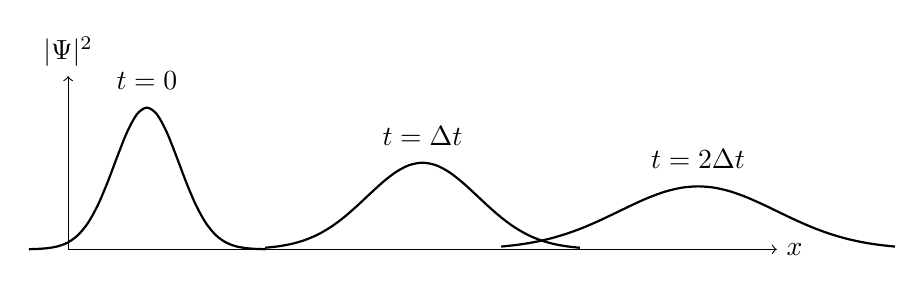
\begin{tikzpicture}[scale=1]
    \draw[->] (-1,0) -- (8,0) node[right] {$x$};
    \draw[->] (-1,0) -- (-1,2.2) node[above] {$|\Psi|^2$};
    \draw[domain=-1.5:1.5, smooth, variable=\x, thick] plot ({\x}, {1.8*exp(-3*\x*\x)});
    \node[above] at (0,1.9) {$t=0$};
    \draw[domain=1.5:5.5, smooth, variable=\x, thick] plot ({\x}, {1.1*exp(-1*(\x-3.5)*(\x-3.5))});
    \node[above] at (3.5,1.2) {$t=\Delta t$};
    \draw[domain=4.5:9.5, smooth, variable=\x, thick] plot ({\x}, {0.8*exp(-0.5*(\x-7)*(\x-7))});
    \node[above] at (7,0.9) {$t=2\Delta t$};
\end{tikzpicture}
\end{center}

O centro avança com velocidade constante $p_0/m$ e a largura cresce com o tempo.

O alargamento da gaussiana pode ser entendido da incerteza inicial na velocidade.

\fbox{\parbox{0.92\textwidth}{
\textbf{Obs:} aproximadamente $\Delta(t) \approx \dfrac{\hbar t}{\Delta}\dfrac{1}{m}$ para $t$ grande.
}}

Saindo da origem em $t=0$:
\begin{equation}
    \left(p_0 - \frac{\hbar}{\Delta}\right)\frac{t}{m} \quad \text{(menor velocidade)} \qquad \left(p_0 + \frac{\hbar}{\Delta}\right)\frac{t}{m} \quad \text{(maior velocidade)}
\label{eq:aula14_velocidades_extremas}
\end{equation}

em $t$ a partícula poderá estar entre

\begin{equation}
    \frac{p_0 t}{m} - \frac{\hbar t}{m\Delta} < x < \frac{p_0 t}{m} + \frac{\hbar t}{m\Delta} \quad \Longrightarrow \quad \Delta x(t) \sim \frac{\hbar t}{m\Delta}
\label{eq:aula14_intervalo_x_t}
\end{equation}

Classicamente você poderia dizer "tenho uma partícula na origem com velocidade $p_0/m$". Em MQ isso não existe. O estado que mais se assemelha a essa condição inicial clássica é exatamente essa gaussiana.

Se a MQ é a teoria correta, por que você nunca viu uma bola de futebol lançada com velocidade $p_0/m$ se tornar cada vez mais "difusa" (correspondendo ao alargamento da gaussiana)?

A razão é que a incerteza em velocidade imposta pela MQ é inobservável para objetos massivos usuais.

\subsubsection*{Quanto à incerteza na velocidade}

Use $\Delta x = 10^{-15}$ m (precisão total na posição)

\begin{equation}
    \Delta p = \frac{\hbar}{2\Delta x} \quad \Longrightarrow \quad \Delta v = \frac{\hbar}{2m\Delta x} =
    \begin{cases}
        5{,}3 \times 10^{-17} \text{ m/s} & (m = 1\text{g}) \\
        5{,}8 \times 10^{10} \text{ m/s} & (\text{elétron})
    \end{cases}
\label{eq:aula14_incerteza_velocidade}
\end{equation}

\subsubsection*{Quanto ao alargamento durante a evolução}

A imprecisão na posição no instante $t$ é da ordem de $(\Delta v)\,t$. Temos que isso se torna igual a 1 mm após

\begin{align}
    1{,}9 \times 10^{13}\ \text{seg} \ (\sim 600.000 \text{ anos}) &\quad \text{para a massa de 1g} \notag \\
    1{,}7 \times 10^{-14}\ \text{seg} &\quad \text{para o elétron}
\label{eq:aula14_tempos_alargamento}
\end{align}

\begin{equation}
    \Longrightarrow \quad \boxed{\text{para partículas do dia-a-dia você NÃO PRECISA tratar o caso livre usando a MQ!!!}}
\label{eq:aula14_conclusao_classica}
\end{equation}

\begin{center}
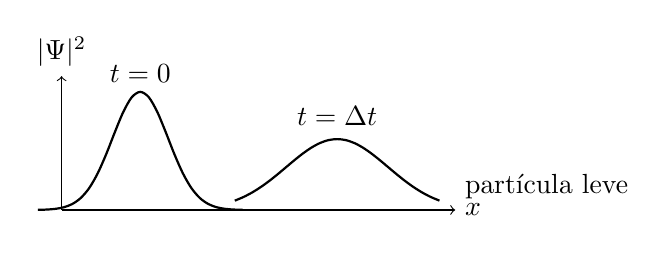
\begin{tikzpicture}[scale=1]
    \draw[->] (-1,0) -- (4,0) node[right] {$x$};
    \draw[->] (-1,0) -- (-1,1.7) node[above] {$|\Psi|^2$};
    \draw[domain=-1.3:1.3, smooth, variable=\x, thick] plot ({\x}, {1.5*exp(-4*\x*\x)});
    \node[above] at (0,1.5) {$t=0$};
    \draw[domain=1.2:3.8, smooth, variable=\x, thick] plot ({\x}, {0.9*exp(-1.2*(\x-2.5)*(\x-2.5))});
    \node[above] at (2.5,0.95) {$t=\Delta t$};
    \node[right] at (4,0.3) {partícula leve};
\end{tikzpicture}

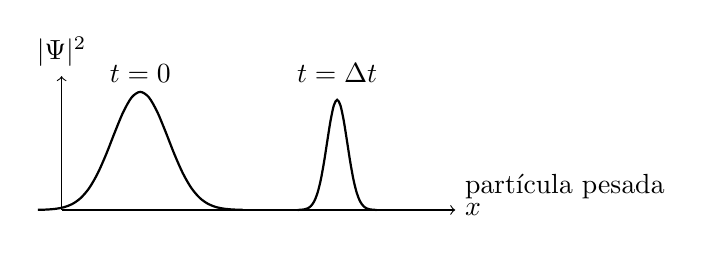
\begin{tikzpicture}[scale=1]
    \draw[->] (-1,0) -- (4,0) node[right] {$x$};
    \draw[->] (-1,0) -- (-1,1.7) node[above] {$|\Psi|^2$};
    \draw[domain=-1.3:1.3, smooth, variable=\x, thick] plot ({\x}, {1.5*exp(-4*\x*\x)});
    \node[above] at (0,1.5) {$t=0$};
    \draw[domain=2.0:3.0, smooth, variable=\x, thick] plot ({\x}, {1.4*exp(-30*(\x-2.5)*(\x-2.5))});
    \node[above] at (2.5,1.5) {$t=\Delta t$};
    \node[right] at (4,0.3) {partícula pesada};
\end{tikzpicture}
\end{center}

Mesmo estado inicial, mesma velocidade média. O alargamento da gaussiana ocorre muito mais rapidamente quando a partícula é leve!

Aqui você vê que para partículas pesadas o que a MQ diz coincide com o que a MC diz. Para todos os efeitos o pacote gaussiano é a partícula clássica, e este se move com a velocidade esperada (\textbf{CONSTANTE}), além de não apresentar alargamento do pacote (que seria algo extremamente bizarro do ponto de vista clássico).

Isso ocorre pois você pode construir um estado quântico com $\Delta x \sim 10^{-15}$ m e $\Delta v \sim 10^{-17}$ m/s, que são incertezas inobserváveis por qualquer instrumento de medida de posição ou velocidade que possam ser construídos.

\subsection*{Pacote livre -- distribuição de momenta}

\begin{equation}
    \Psi(x,t) = \frac{1}{\pi^{1/4}\Delta^{1/2}f^{1/2}}\, \exp\left[-\frac{(x-p_0t/m)^2}{2\Delta^2 f} + \frac{ip_0 x}{\hbar} - \frac{ip_0^2}{2m}\frac{t}{\hbar}\right]
\label{eq:aula14_psi_xt_compacta}
\end{equation}
onde
\begin{equation}
    f = 1 + \frac{i\hbar t}{m\Delta^2}
\label{eq:aula14_f_def}
\end{equation}

\begin{equation}
    |\Psi(x,t)|^2 = \frac{1}{\sqrt{\pi}\,\Delta\,|f|}\, \exp\left[-\frac{(x-p_0t/m)^2}{\Delta^2|f|^2}\right] \qquad \text{(densidade de prob. de posição)}
\label{eq:aula14_densidade_prob_f}
\end{equation}

Podemos calcular também (tomando a transformada de Fourier de $\Psi(x,t)$)

\begin{align}
    \widetilde{\Psi}(p,t) &= \left(\frac{\Delta}{\hbar}\right)^{1/2} \frac{1}{\pi^{1/4}}\, \exp\left[-\frac{(p-p_0)^2\Delta^2 f}{2\hbar^2} + \frac{i(p_0-p)p_0t}{\hbar m} - \frac{ip_0^2}{2m}\frac{t}{\hbar}\right] \label{eq:aula14_fourier_p_passo1} \\
    &= \left(\frac{\Delta}{\hbar}\right)^{1/2} \frac{1}{\pi^{1/4}}\, \exp\left[-\frac{(p-p_0)^2\Delta^2}{2\hbar^2} - \frac{ip^2}{2m}\frac{t}{\hbar}\right] \label{eq:aula14_fourier_p_passo2}
\end{align}

\begin{equation}
    |\widetilde{\Psi}(p,t)|^2 = \frac{\Delta}{\hbar\sqrt{\pi}}\, \exp\left[-\frac{(p-p_0)^2\Delta^2}{\hbar^2}\right] \qquad \text{(densidade de prob. de MOMENTO)}
\label{eq:aula14_densidade_prob_momento}
\end{equation}

Note que a distribuição de momenta $|\widetilde{\Psi}(p,t)|^2$ permanece constante enquanto $|\Psi(x,t)|^2$ se alarga.

Isso era de se esperar, pois:

\begin{equation}
    \ket{\Psi(t)} = e^{-i\hat{H}t/\hbar}\ket{\Psi(0)}
\label{eq:aula14_psi_t_op}
\end{equation}

\begin{align}
    \bra{p}\Psi(t)\rangle &= \bra{p}e^{-i\hat{H}t/\hbar}\ket{\Psi(0)} \notag \\
    &= e^{-i\frac{p^2t}{2m\hbar}}\braket{p}{\Psi(0)} \quad \Longrightarrow \quad |\widetilde{\Psi}(p,t)|^2 = |\widetilde{\Psi}(p,0)|^2
\label{eq:aula14_invariancia_momento}
\end{align}
